\documentclass[tikz,border=10pt]{standalone}
\usepackage{tikz}
\usepackage[T1]{fontenc}
\usetikzlibrary{positioning, arrows.meta}

\begin{document}
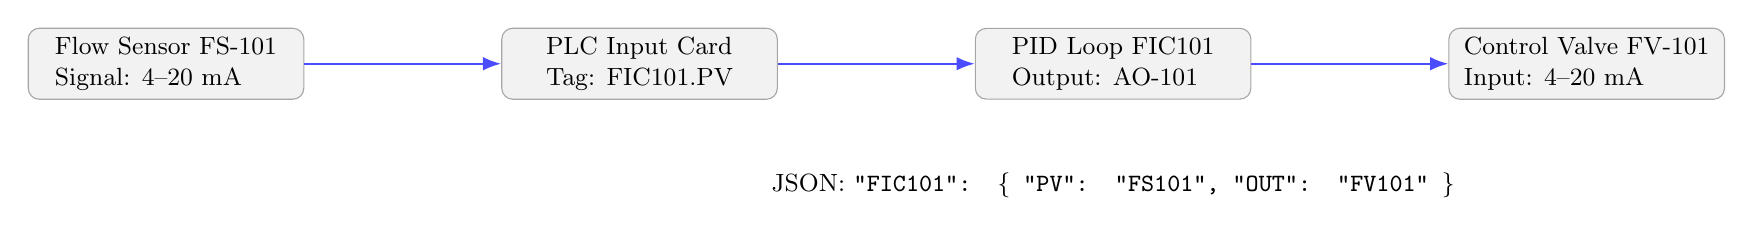
\begin{tikzpicture}[node distance=1cm, font=\small,
  io/.style={rectangle, rounded corners, draw=gray!70, fill=gray!10, minimum width=3.5cm, align=left},
  arrow/.style={-Latex, thick, blue!70}
]

\node[io] (sensor) {Flow Sensor FS-101\\Signal: 4–20 mA};
\node[io, right=2.5cm of sensor] (plc) {PLC Input Card\\Tag: FIC101.PV};
\node[io, right=2.5cm of plc] (controller) {PID Loop FIC101\\Output: AO-101};
\node[io, right=2.5cm of controller] (valve) {Control Valve FV-101\\Input: 4–20 mA};

\draw[arrow] (sensor) -- (plc);
\draw[arrow] (plc) -- (controller);
\draw[arrow] (controller) -- (valve);

\node[below=0.8cm of controller] (note)
  {JSON: \texttt{"FIC101": \{ "PV": "FS101", "OUT": "FV101" \}}};


\end{tikzpicture}
\end{document}
